\chapter{The CF Pumping Lemma, Turing Machines}

\section{Non-context-free languages}

Based on \hyperref[theorem: CFG=PDA]{the equivalence of CFGs and PDAs}, there are some more corollaries we can see or easy to prove:

\begin{corollary}
    Every regular language is a CFL
\end{corollary}

\begin{corollary}
    If \(A\) is a CFL and \(B\) is regular then \(A \cap B\) is a CFL. 

    \begin{example}
        A: \(A = \{ a^nb^n | n \geq 0\} \) 
        B: \(B = \{ (ab)^* \} \) 
    \end{example}

    Proof sketch: while reading the input, the finite control of the PDA for \(A\) simulates the DFA for \(B\).  
\end{corollary}

Need to notice that the class of CFLs is not closed under \(\cap\) which is different from regular languages.

\begin{example}
    I will show an example where the intersection of 2 CFLs is not a CFL.

    \(L_1 = \{ a^n b^n c^m | n, m \geq 0 \} \) 

    \(L_2 = \{ a^m b^n c^n | n, m \geq 0 \} \) 

    \(L_1 \cap \L2 = \{ a^n b^n c^n | n \geq 0\} \) 

    Intuitively, to recognize the intersection of \(L_1\) and \(L_2\) we need to compare the count of \(a, b, c\). One stack can only handle the comparison of \(a\) and \(b\), but we have no extra stack for comparing \(c\).      
\end{example}

But the class of CFLs is closed under \(\cup, \circ, *\).  
\begin{note}
    Should try to prove its closed under union, concatenation and star!
\end{note}

\subsection{CF Pumping Lemma}
To prove a language is \textbf{not context free}, we need another tool:
\begin{example}\label{eg: 5.1}
    Let \(B = \{ 0^k 1^k 2^k | k \geq 0\} \), we will show that B is not a CFL. 
\end{example}

The tool we'll use is \textbf{Pumping Lemma for CFLs}: 
\begin{lemma}[Pumping Lemma for CFLs]
    If \(A\) is a CFL, then there is a number \(p\)(the pumping length) where, if \(s\) is any string in \(A\) of length at least \(p\), 
    then \(s\) may be divided into \textcolor{red}{five pieces \(s = uvxyz\)} satisfying the conditions
    \begin{enumerate}
        \item for each \(i \geq 0\), \(uv^i xy^iz \in A\)
        \item \(|vy| > 0\)
        \item \(|vxy| \leq p\)   
    \end{enumerate}    
\end{lemma}
\begin{proof}
    \begin{intuition}
    
    Proof IDEA: let \(s\) be a \textit{very long} string in \(A\), then the parsing tree for \(s\) must be very tall.  
    Then the parse tree must contain some long path from the start variable to the terminal symbol at a leaf. 
    On this long path, because of the pigeonhole principle, some variable \(R\) must repeat. 

    \begin{figure}[H]
        \centering
        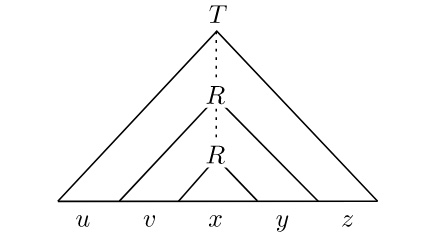
\includegraphics[width=0.6\textwidth]{f2.35-1.jpg}
        \caption{when \(s = uvxyz\) }
    \end{figure}

    This repetition allows us to replace the subtree under the second occurrence of \(R\) with the subtree under the first occurrence of \(R\) and still get a legal parse tree.  

    \begin{figure}[H]
        \centering
        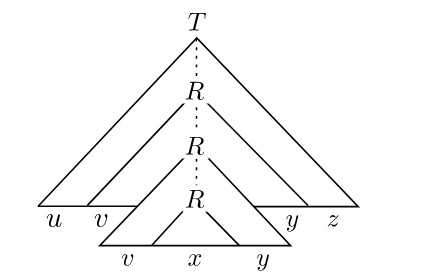
\includegraphics[width=0.6\textwidth]{f2.35-2.jpg}
        \caption{when \(s = uv^i xy^i z\) }
    \end{figure}

    Also \(v\) and \(y\) can repeat 0 time:

    \begin{figure}[H]
        \centering
        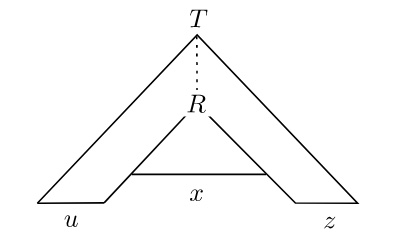
\includegraphics[width=0.6\textwidth]{f2.35-3.jpg}
        \caption{when \(s = uxz\) }
    \end{figure}
    \end{intuition}
\end{proof}

Let's go back to the \hyperref[eg: 5.1]{example}:
\begin{example}
    \(B = \{ 0^k1^k2^k | k \geq 0 \} \) 

    Proof by Contradiction:
    Assume that B \underline{is} a CFL.

    Based on CFL pumping lemma gives \(p\) as above, Let \(s = 0^p1^p2^p \in B\).  

    Pumping lemma says that can divide \(s = uwxyz\) satisfying the 3 conditions. 

    Condition 3 (\(|vxy| \leq p\)) implies that \(vxy\) can not contain both 0s and 2s. 

    So \(uv^2xy^2z\) has unequal numbers of 0s, 1s and 2s.
\end{example}

Another example:
\begin{example}
    Let \(F = \{ ww|w \in \Sigma^* \} \). \(\Sigma = \{ 0, 1 \} \). 
    
    Show: F is not a CFL.  

    Suppose \(F\) is a CFL, we try to construct a string which violate the CFL pumping lemma. 

    \begin{itemize}
        \item Try \(s_1 = 0^p10^p1\), we can choose \(x = 1\) of the middle, and v and y the left and right 0, and we can pump to this string. 
        \(\rightarrow\) \textcolor{red}{This is a bad choice to try to find a contradiction} 
        \item Try \(s_2 = 0^p 1^p 0^p 1^p\), now we can find the contradiction!
    \end{itemize}
\end{example}

\section{Turing Machines(TMs)}

Finite automata are good models for devices that have a small amount of memory. Pushdown automata are good models for devices that have an unlimited memory that is usable only in the last in, first out manner of stack.

We also have shown that some very simple tasks are beyond the capabilities of the models.

Alan Turing propose Turing Machine in 1936, it's similar to a finite machine but with an \textbf{unlimited and unstricted memory}. It is a much more accurate model of a general purpose computer. \textit{A Turing machine can do anything that a real computer can do, but even a Turing machine cannot solve certain problems.}

\begin{figure}[H]
    \centering
    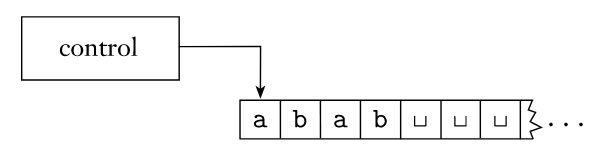
\includegraphics[width=0.8\textwidth]{f3.1.jpg}
    \caption{Schematic of a Turing machine}
\end{figure}

Important characteristics of it:
\begin{enumerate}
    \item Head can read and write
    \item Head is two way (can move left or right)
    \item Tape is infinite (to the right)
    \item Infinitely many blank follow input
    \item Can accept or reject any time (not only at end of input)
\end{enumerate}


\begin{example}
    TM recognizing \(B = {a^k b^k c^k | k \geq 0}\):

    Example: \verb|aaabbbccc␣␣| 

    \begin{enumerate}
        \item Scan right until ␣ while checking if input is in \(a^*b^*c^*\), \(reject\) if not
        \item Return head to left  
        \item Scan right, crossing off single a, b and c: \(\cancel{a}aa\cancel{b}bb\cancel{c}cc\) 
        \item If the last one of each symbol, \(accept\)
        \item If the last one of some symbol but not others, \(reject\)
        \item If all symbols remain, return to left and repeat from step 3.  
    \end{enumerate}

    After step 6, it will go back to step 3, and the string will become \(\cancel{a}\cancel{a}a\cancel{b}\cancel{b}b\cancel{c}\cancel{c}c\).
    Then go to step 4, they are all last one of each symbol, so we \(accept\). 

    The effect of "crossing off" is brought by use a tape alphabet like \(\Gamma = \{ a, b, c, \cancel{a}, \cancel{b}, \cancel{c}, \sqcup \} \). 
\end{example}

\begin{definition}[Turing Machine]
   A Turing Machine (TM) is a 7-tuple \((Q, \Sigma, \Gamma, \sigma, q_0, q_{acc}, q_{rej})\). 

   \begin{itemize}
    \item \(\Sigma\) input alphabet
    \item \(\Gamma\) tape alphabet (\(\Sigma \subseteq \Gamma\))
    \item \(Q \times \Gamma \rightarrow Q \times \Gamma \times \{ L, R \} \) \quad (L = left, R = right)  
   \end{itemize}

   The transition function means that the head in a certain state \(q\) and the head is over a tape square containing a symbol \(a\). 
   And if \(\delta(q, a) = (r, b, L)\), the machine writes the symbol \(b\) replacing \(a\), and goes to state \(r\). The third L means the head moves to left after writing.    
\end{definition}

On input \(w\) a TM \(M\) may halt (enter \(q_{acc}\) or \(q_{rej}\)) or \(M\) may run forever ("loop"). 

So \(M\) has 3 possible outcomes for each input \(w\):
\begin{enumerate}
    \item \underline{Accept} \(w\) (enter \(q_{acc}\)) 
    \item \underline{Reject} \(w\) by halting(enter \(q_{rej}\)) 
    \item \underline{Reject} \(w\) by looping (running forever) 
\end{enumerate}  

The above definition of TM is \textbf{deterministic}, but we can change it to be \textbf{nondeterministic} by change \(\delta\) to \(\delta: Q \times \Gamma \rightarrow \P(Q \times \Gamma \times \{ L, R \}) \)  

\subsection{TM recognizers and deciders}

\begin{definition}
    A is \underline{Turing-recognizable} if \(A = L(M)\) for some TM \(M\).  
\end{definition}

\begin{definition}
    TM \(M\) is a \underline{decider} if \(M\) halts on all inputs. (no looping, meaning eventually the machine will halt to \(q_{acc}\) or \(q_{rej}\))  
\end{definition}

\begin{definition}
    \(A\) is \underline{Turing-decidable} if \(A = L(M)\) for some TM decider \(M\).    
\end{definition}

A Turing recognizable language can cause the machine reject by looping, but a Turing decidable language can always call the TM halt, thus we have the relationship:

\begin{figure}[H]
    \centering
    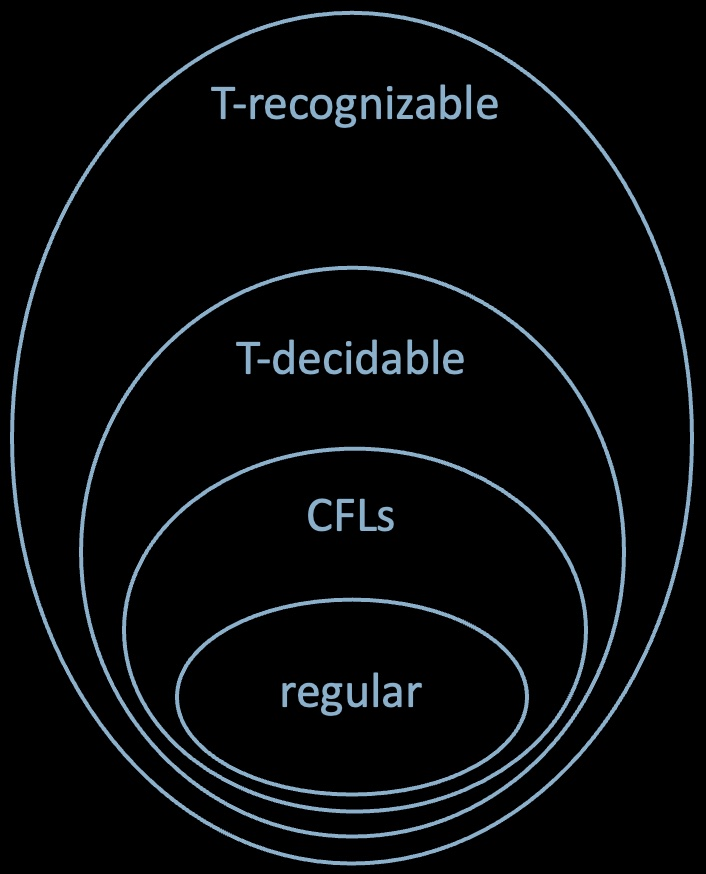
\includegraphics[width=0.8\textwidth]{l5.1.jpg}
    \caption{Summary of languages}
\end{figure}